\section{Advanced Control Flow Issues}
\label{sec:advancedissues}
%In chapter \ref{chap:translation} we described the techniques necessary to generate code from the producer-consumer ProPCPN model. We described in detail how the model was decorated, and then translated into a control flow graph (CFG). The CFG was then translated into an abstract syntax tree (AST) representing a simple language we designed for the purpose. Then we choose the functional language Erlang as the target language, i.e., created an Erlang syntax tree (EST) which could be pretty printed into a textual representation of the program. 

While covering most of the construct found in ProPCP-nets, the producer-consumer model does not contain a branch of the control flow. In this section we describe how branches of control flow are handled in the translation. In the producer-consumer model process tokens residing on a process place are only available to a single transition. The definition allows process tokens to be available to multiple transitions, i.e., a control flow branch. Having control flow branches introduce an additional challenge when the target transitions have input arcs from buffer places. These buffer places have to be taken into consideration when choosing the flow of control. Making a function call without looking at the buffer may introduce a deadlock in the program that did not exist in the model.

\subsection{Control Flow Branches}

\begin{figure}[b!]
\centering
\includegraphics[scale=0.5]{translation/advancedissues/graphics/cffcpn.eps}
\caption{A process partition with a control flow branch}
\label{fig:cffcpn}
\end{figure}

In Fig.~\ref{fig:cffcpn} we see part of a ProPCPN model with one process place \figitem{Process Place}, two transitions \figitem{T1} and \figitem{T2}, and two buffer places \figitem{Buffer1} and \figitem{Buffer2}. The process token can either be removed by \figitem{T1} or \figitem{T2}, and are in both cases, put back on \figitem{Process Place}. \figitem{T1} is enabled if \figitem{guard1} evaluates to \code{true} and there is a token on \figitem{Buffer1}, and analogously for \figitem{T2}. This means that the generated process can proceed to either \figitem{T1} or \figitem{T2} depending on them being enabled.

\subsubsection{Translating to a CFG} 

Given the ProPCPN model shown in in Fig.~\ref{fig:cffcpn} we generate the CFG shown in Fig.~\ref{fig:cffcfg}. It contains an entry basic block \code{start} which has an edge with the condition \code{guard1} to the basic block \code{T1}, and an edge with the condition \code{guard2} to the basic block \code{T2}.
%The label represents (as explained in section \ref{sec:cpntranslation}) the condition for the flow in that direction.
The flow of control from \code{T1} is either to itself, or to \code{T2} depending on the value of \code{guard1} and \code{guard2}, and analogously for \code{T2}. \code{T1} contains a receive statement from \code{Buffer1} and \code{T2} contains a receive statement from \code{Buffer2}. 

\begin{figure}
\centering
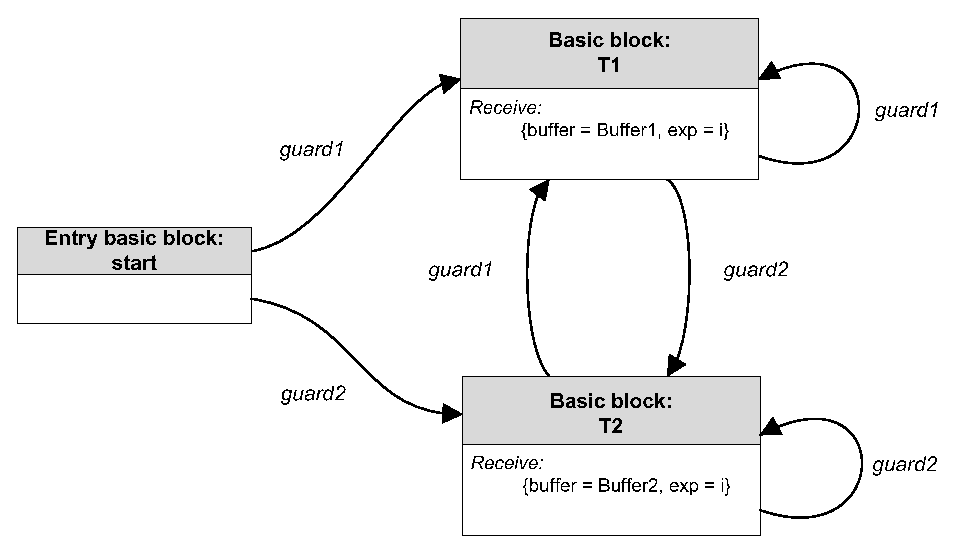
\includegraphics[scale=0.5]{translation/advancedissues/graphics/cffcfg.eps}
\caption{The CFG showing the control flow branch}
\label{fig:cffcfg}
\end{figure}

\subsubsection{Translating to an AST}

The CFG is then translated to the AST shown in Fig.~\ref{fig:cffast}. The \code{Process} node contains two blocks \code{T1} and \code{T2}. Taking a look at \code{T1} it contains a receive statement which has a pointer to \code{Buffer1} where the incoming messages are stored. The receive statement also contains a local variable \code{i} into which a message from the buffer is read. \code{T1} also contains two conditional statements; one holding the condition expression \code{guard1} and pointing to \code{T1}, and one holding the condition expression \code{guard2} and pointing to \code{T2}. The block \code{T2} is similar to \code{T1}.

\begin{figure}[b!]
\centering
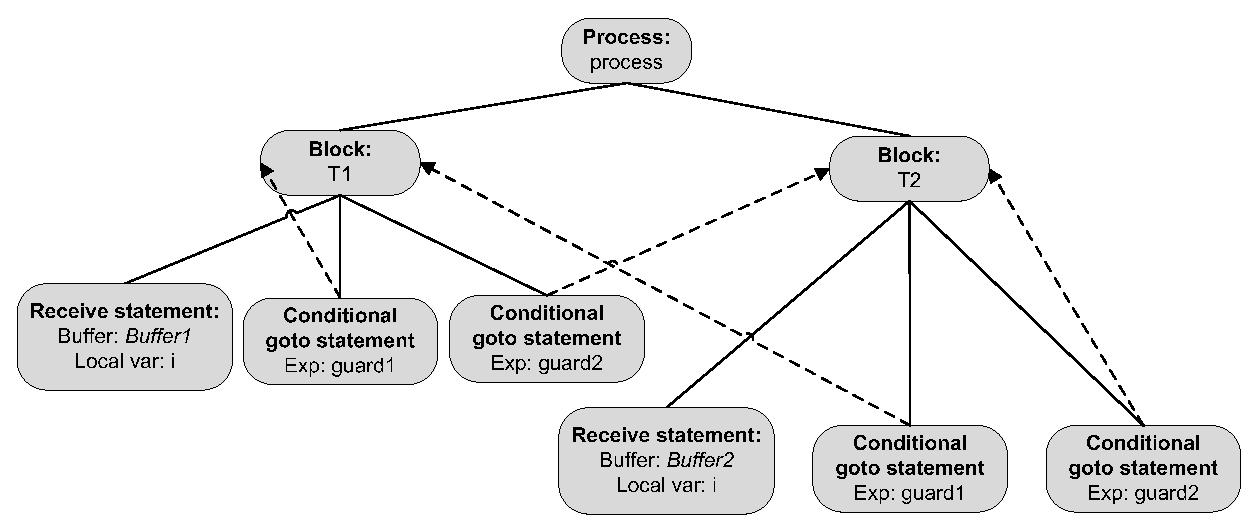
\includegraphics[scale=0.65]{translation/advancedissues/graphics/cffast.eps}
\caption{The AST showing the control flow branch}
\label{fig:cffast}
\end{figure}

\subsubsection{Translating to Erlang Source Code}
%In the phase from AST to EST things become a bit more complicated when buffers are involved as in this small example.
Next, we explain how control flow branches are handled when there are no buffers involved. In this section we omit the EST and only show the printed Erlang code. In Listing~\ref{list:cffnobuf} we see the code for \code{t1} generated from the AST (ignoring the receive statements) in Fig.~\ref{fig:cffast}.

\begin{figure}[h!]
\begin{verbatim}[style=erlangcode, caption=Generated Erlang code without receive statements, label=list:cffnobuf]
t1() -> 
    ...
    if
        Guard1 ->
            t1();
        Guard2 ->
            t2()
    end.
\end{verbatim}
\end{figure}


In the bottom of the function the guard expressions are evaluated, and jumps are made accordingly. Notice that if none of the guard expressions evaluate to \code{true} the program terminates. This is equivalent to the behaviour of the CPN model, in which this corresponds to none of the transitions, the process can proceed to, being enabled. Since we do not allow tokens on shared places or buffer places to be referred to in the guard expressions, the transitions cannot become enabled in the future.

This is code is generated for control flow branches when the goto statements points to blocks without receive statements. Generating Erlang code when there is a receive statement in one of the target blocks is a bit more complicated.

\paragraph{Goto a block with a receive statement.}
Jumping to the first block were the guard evaluates to \code{true} could introduce a deadlock in the program if that block contains a receive statement from a buffer that will never have an element added. For instance, in the ProPCPN model shown in fig.~\ref{fig:cffcpn}, it could be the case that both \figitem{guard1} and \figitem{guard2} evaluates to \code{true}. Assume that \figitem{Buffer1} is empty, and that there will never be added a token to it. Assume also that \figitem{Buffer2} already contains a token. If the program where to jump to the function corresponding to the transition \figitem{T1} the program would stop on the blocking receive expression. This is not desirable since \figitem{T2} is enabled in the CPN model, thus calling the function corresponding to \figitem{T2}, would not make the program stop.

The solution we have found is to only jump to a function with a receive expression if there is an element in the buffer. Since buffers are local to a process instance, the element will remain in the buffer until removed by that process instance. Thus it is guaranteed that the buffer element is still available when the function will be executed. We have introduced an explicit Erlang buffer module (found in appendix \ref{appsec:buffer}) with two additional operations:

\begin{itemize}
 \item The function \code{has\_element} can be used to determine if there is an element in the buffer. It does not change the state of the buffer. 
 \item The function \code{interrupt\_me} is used like a blocking receive call if the buffer is empty. The buffer will send a message with the atom literal \code{interrupt} when an element is added to the buffer.
\end{itemize}

\begin{figure}[h!]
\begin{verbatim}
    t1(Env) -> 
    ...
    t1_loop(Env).

t1_loop(Env) -> 
    Env#environment.buffer_1 ! has_element,
    receive 
        Buffer_1_has_elements -> 
            Buffer_1_has_elements
    end,
    Env#environment.buffer_2 ! has_element,
    receive 
        Buffer_2_has_elements -> 
            Buffer_2_has_elements
    end,
    if
        Guard1, Buffer_1_has_elements ->
            t1(Env); 
        Guard2, Buffer_2_has_elements ->
            t2(Env);
        true ->
            if
                not Buffer_1_has_elements ->
                    Env#environment.buffer_1 ! interrupt_me;
            end,       
            if       
                not Buffer_2_has_elements ->
                    Env#environment.buffer_2 ! interrupt_me
            end
    end,
    receive 
        interrupt -> 
            t1_loop(Env)
    end.
\end{verbatim}
\end{figure}


Listing~\ref{list:cffwithbuf} shows how \code{has\_element} and \code{interrupt\_me} are used in the generated code. The function \code{t1\_loop} line 5-34 is used to decide which function to call next. In line 6-15 the \code{has\_element} operation is used on \code{Buffer1} and \code{Buffer2} and bound to variables. In line 17-18 we see how the function \code{t1} is called if \code{Guard1} evaluates to \code{true} and the buffer has an element. The \code{true} branch in line 21-29 is used if no function is available, i.e., none of the above guards evaluates to \code{true} or the buffers had no elements. This means, that until one of the buffers receives an element, none of the functions can be called. For this reason, it is requested that all the buffers without elements make an interrupt when an element becomes available. Finally, in line 31-34 \code{t1} is blocked until an interrupt is received from one of the buffers, in which case \code{t1\_loop} is called again.
